\tikzset{%
    every neuron/.style={
        circle,
        draw,
        minimum size=5pt,
        inner sep=0pt,
        very thin
    },
    neuron/.style={
        fill
    },
}
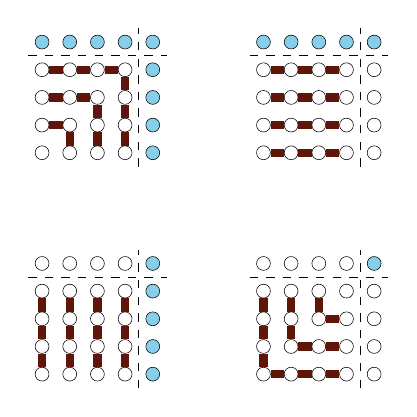
\begin{tikzpicture}[x=0.8cm, y=0.8cm, >=latex, every text node part/.style={align=center}]
    \foreach \x in {0,...,3}
        \foreach \y in {0,...,3} {
            \pgfmathtruncatemacro{\label}{\x*10+\y}
            \node [every neuron/.try] (\label) at (10pt*\x,10pt*\y) {};
        } 
    \foreach \x/\y in {4/0, 4/1, 4/2, 4/3} {
        \node [every neuron/.try, fill=SkyBlue] () at (10pt*\x,10pt*\y) {};
    }
    \foreach \x/\y in {0/4, 1/4, 2/4, 3/4, 4/4} {
        \node [every neuron/.try, fill=SkyBlue] () at (10pt*\x,10pt*\y) {};
    }
    \path[dashed] (-5pt, 35pt) edge (45pt, 35pt);
    \path[dashed] (35pt, -5pt) edge (35pt, 45pt);
    \path[Sepia, line width=3pt] (1) edge (11);
    \path[Sepia, line width=3pt] (11) edge (10);
    \path[Sepia, line width=3pt] (2) edge (12);
    \path[Sepia, line width=3pt] (12) edge (22);
    \path[Sepia, line width=3pt] (22) edge (21);
    \path[Sepia, line width=3pt] (21) edge (20);
    \path[Sepia, line width=3pt] (3) edge (13);
    \path[Sepia, line width=3pt] (13) edge (23);
    \path[Sepia, line width=3pt] (23) edge (33);
    \path[Sepia, line width=3pt] (33) edge (32);
    \path[Sepia, line width=3pt] (32) edge (31);
    \path[Sepia, line width=3pt] (31) edge (30);

    \foreach \x in {0,...,3}
        \foreach \y in {0,...,3} {
            \pgfmathtruncatemacro{\label}{1000+\x*10+\y}
            \node [every neuron/.try] (\label) at (10pt*\x+80pt,10pt*\y) {};
        } 
    \foreach \x/\y in {4/0, 4/1, 4/2, 4/3} {
        \node [every neuron/.try, fill=white] () at (10pt*\x+80pt,10pt*\y) {};
    }
    \foreach \x/\y in {0/4, 1/4, 2/4, 3/4, 4/4} {
        \node [every neuron/.try, fill=SkyBlue] () at (10pt*\x+80pt,10pt*\y) {};
    }
    \path[dashed] (75pt, 35pt) edge (125pt, 35pt);
    \path[dashed] (115pt, -5pt) edge (115pt, 45pt);
    \foreach \x in {0,...,2}
        \foreach \y in {0,...,3} {
            \pgfmathtruncatemacro{\label}{1000+\x*10+\y}
            \pgfmathtruncatemacro{\labell}{1000+\x*10+\y+10}
            \path[Sepia, line width=3pt] (\label) edge (\labell);
        }

    \foreach \x in {0,...,3}
        \foreach \y in {0,...,3} {
            \pgfmathtruncatemacro{\label}{2000+\x*10+\y}
            \node [every neuron/.try] (\label) at (10pt*\x,10pt*\y-80pt) {};
        } 
    \foreach \x/\y in {4/0, 4/1, 4/2, 4/3, 4/4} {
        \node [every neuron/.try, fill=SkyBlue] () at (10pt*\x,10pt*\y-80pt) {};
    }
    \foreach \x/\y in {0/4, 1/4, 2/4, 3/4} {
        \node [every neuron/.try, fill=white] () at (10pt*\x,10pt*\y-80pt) {};
    }
    \path[dashed] (-5pt, -45pt) edge (45pt, -45pt);
    \path[dashed] (35pt, -85pt) edge (35pt, -35pt);
    \foreach \x in {0,...,3}
        \foreach \y in {0,...,2} {
            \pgfmathtruncatemacro{\label}{2000+\x*10+\y}
            \pgfmathtruncatemacro{\labell}{2000+\x*10+\y+1}
            \path[Sepia, line width=3pt] (\label) edge (\labell);
        }

    \foreach \x in {0,...,3}
        \foreach \y in {0,...,3} {
            \pgfmathtruncatemacro{\label}{3000+\x*10+\y}
            \node [every neuron/.try] (\label) at (10pt*\x+80pt,10pt*\y-80pt) {};
        } 
    \foreach \x/\y in {4/0, 4/1, 4/2, 4/3} {
        \node [every neuron/.try, fill=white] () at (10pt*\x+80pt,10pt*\y-80pt) {};
    }
    \foreach \x/\y in {0/4, 1/4, 2/4, 3/4} {
        \node [every neuron/.try, fill=white] () at (10pt*\x+80pt,10pt*\y-80pt) {};
    }
    \foreach \x/\y in {4/4} {
        \node [every neuron/.try, fill=SkyBlue] () at (10pt*\x+80pt,10pt*\y-80pt) {};
    }
    \path[dashed] (75pt, -45pt) edge (125pt, -45pt);
    \path[dashed] (115pt, -85pt) edge (115pt, -35pt);
    \path[Sepia, line width=3pt] (3032) edge (3022);
    \path[Sepia, line width=3pt] (3022) edge (3023);
    \path[Sepia, line width=3pt] (3031) edge (3021);
    \path[Sepia, line width=3pt] (3021) edge (3011);
    \path[Sepia, line width=3pt] (3011) edge (3012);
    \path[Sepia, line width=3pt] (3012) edge (3013);
    \path[Sepia, line width=3pt] (3030) edge (3020);
    \path[Sepia, line width=3pt] (3020) edge (3010);
    \path[Sepia, line width=3pt] (3010) edge (3000);
    \path[Sepia, line width=3pt] (3000) edge (3001);
    \path[Sepia, line width=3pt] (3001) edge (3002);
    \path[Sepia, line width=3pt] (3002) edge (3003);
\end{tikzpicture}